\section{Matrículas}

Com exceção das matrículas de época, os formatos das matrículas devem ser
utilizados de acordo com a data da matriculação em Portugal. Podem-se utilizar
matrículas de formatos mais recentes, mas não se podem utilizar formatos
anteriores, sob pena de autuação pelas autoridades.

\begin{figure}[htbp]
  \centering
  \begin{tabular}{@{}c c@{}}
    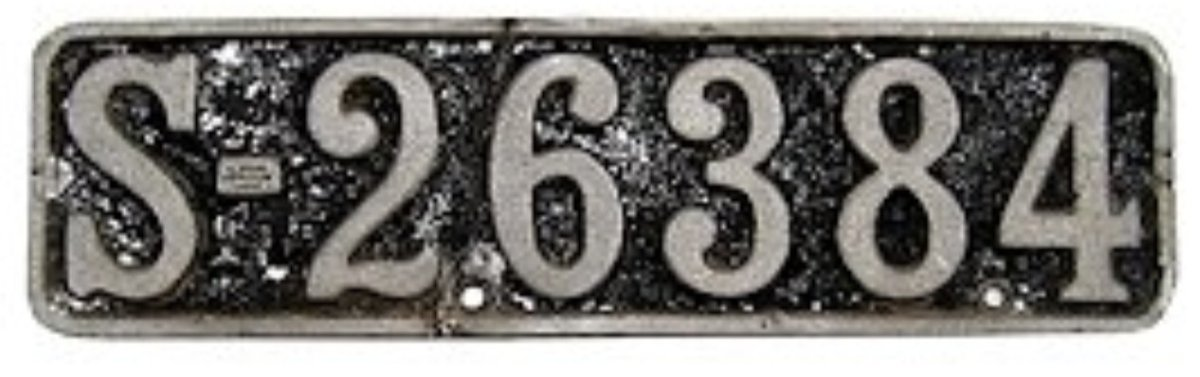
\includegraphics[height=1.3cm]{fmt-1911} & 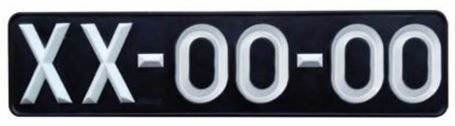
\includegraphics[height=1.3cm]{fmt-1937} \\
    \small 1911 a 31/12/1936 & \small 1/1/1937 a 31/12/1991 \\[0.6em]
    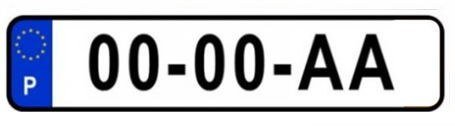
\includegraphics[height=1.3cm]{fmt-1992} & 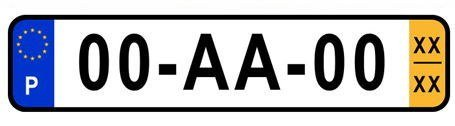
\includegraphics[height=1.3cm]{fmt-2005} \\
    \small 1/1/1992 a 31/12/1997 & \small 1/1/1998 a 2/3/2020 \\[0.6em]
    \multicolumn{2}{c}{
\includegraphics[height=1.3cm]{fmt-2020}} \\
    \multicolumn{2}{c}{\small A partir de 3/3/2020}
  \end{tabular}
  \caption{Os cinco formatos de matrícula e o período em que cada aparência foi atribuída. A edição de 2023 indicava 31/12/2019 e 1/1/2020. O Decreto-Lei n.º 2/2020
liga o novo modelo de chapa ao início da emissão do novo formato, e a primeira
matrícula \plate{AA 01 AA} foi emitida a 3 de março de 2020 (IMT).}
\end{figure}

As chapas de matrícula mais recentes seguem o modelo europeu: cor branca
refletora como base, caracteres a preto. No lado esquerdo é colocada a banda
azul (“eurobanda”) com a letra de identificação nacional: \plate{P}.

No lado direito, até à última alteração, surgia a barra amarela com a indicação
do mês e do ano do primeiro registo do veículo (por exemplo, um carro de junho
de 1997 teria indicado \plate{97/06}).

Mas se o carro foi matriculado antes de 1 de janeiro de 1998, pode usar o modelo
em vigor à data da matrícula, ou seja:
\begin{itemize}
  \item chapas pretas com caracteres brancos para os que foram matriculados até
        31 de dezembro de 1991;
  \item chapas brancas com a eurobanda azul, mas sem a barra amarela, para os
        veículos matriculados entre 1 de janeiro de 1992 e 31 de dezembro de 1997.
\end{itemize}

Os veículos antigos considerados de interesse museológico podem usar uma chapa do
modelo em vigor quando entraram em circulação. Os automóveis têm duas chapas, uma
à frente e outra atrás (Decreto-Lei n.º~54/2005, art.~7.º; ver a
secção~\ref{sec:legislacao}).

\needspace{14\baselineskip}
\gen{series}
